\begin{quoting}
\todo[inline]{Find a nice quote here}
\end{quoting}

Nowadays the vast market of mobile and embedded devices is growing much faster than the traditional PC or server markets. With many more new use cases being implemented and researched, one can see an explosion in a number of devices, their security requirements and platform security mechanisms. In order not to get lost in this constantly evolving variety, it is important to define a \textit{generic platform security model} that can be used for classifying different types of security mechanisms and techniques, as well as compare platform security architectures between each other. 

Publication I of this thesis, as well as the related Publication VII (not included in this thesis), focus on on creating this platform security model and comparing existing mobile platform architectures based on it. At the time of writing, mobile platforms were the most prominent direction for the OS platform security research and this explains the focus of the publications. The platform security model, defined in Publication VII is built on top of a set of common design patterns described in Publication I. These include hardware-assisted security mechanisms (secure boot, trusted execution environment, sealing and attestation, etc.) described in Section III of Publication I, as well as software-only security mechanisms (protection of application integrity, run-time access control and permission assignment etc.), described in Section VI of Publication I. The history of many of these design patterns go back some decades ago and they are constantly reused in newly coming platform security designs as the "best known method" to fulfill a certain set of security requirements. For example, the "\textit{measure-before-execute}" design principle that is a foundation of the secure boot mechanism is a robust method to ensure that the software boot chain is free from offline (potentially malicious) modifications. Moreover, the first efforts to define and use hardware-assisted security mechanisms in platform security designs go back to late 1990s when the Trusted Computing Platform Alliance (TCPA)~\cite{pearson2002} defined the first hardware-assisted elements for PCs.

There are four different mobile platforms that are discussed in Publication I: Symbian, Java ME, Android and MeeGo. This set is further extended to six in Publication VII by adding iOS and Windows Phone to the comparison. All of these platforms are compared in terms of security mechanisms they support, both hardware-assisted and software-only. However, as history has shown, only two of these mobile OSes have managed to reach significant device volumes in modern days, namely Android and iOS (73.5\% and 19.9\% of mobile market share respectively~\cite{osshare}). Both of these platforms preserve their overall platform security models, described in Publications I and VII, and some valuable new security mechanisms have been added over time, as well as existing ones improved. 

The Android platform saw a major usage growth and strengthing of its Mandatory Access Control mechanism, SEAndroid~\cite{smalley12} (a variant of SELinux). Starting from Android 5.0 SEAndroid is mandatory for OEMs to use and enable in the enforcing mode. The Security HW API, previously very limited to the secure storage functionality only, now is fully changed to an extensive and powerful \textit{Trusty TEE API}~\cite{trusty} that can be used as an interface towards Security HW. Android has also started to support various device encryption methods~\cite{androidencr} in order to guarantee confidentiality of user's data: the full disk encryption and the file-based encryption were added in Android 5.0 and 7.0 releases respectively. The newly added hardware-backed keystore, Keymaster~\cite{androidkeymaster}, allows applications to take advantage of various cryptographic primitives and have their keys securely stored by underneath security HW. Since Android 7.0 Keymaster also supports \textit{key attestation} and \textit{version binding}, where it is possible to bind keys to a specific version of OS or even patch version. 

\todo[inline]{here tell about iOS changes since publication VI: this needs more studying since I have not worked with iOS at all} 

As we extend our focus from mobile devices to the embedded and IoT world, the situation changes: there is no more a single software platform or OS that dominates this market. This is due to the very different nature of how embedded devices are designed and produced by OEMs, as well as to a much wider set of use cases that such devices must support, such as automation, automotive, healthcare etc. A typical embedded device is usually a single purpose device, i.e. light sensor, garage door controller, factory supervision drone, but depending on the purpose can have very different hardware and software stacks. For example, a device might need to interact with a user and therefore require a user interface or it might not need one at all. Similar with other technology support, as TCP/IP networking, Bluetooth, wireless, etc. Moreover, embedded devices differ greatly in their HW capabilities: from very low-end devices having only KB of memory to high-end devices no different than a typical mobile or PC platform.

Thus there is not a single ready-build OS that would serve as a good fit for all of these different purposes without causing an overhead of unnecessary components. Instead, in the embedded world, it is more common to use an "\textit{OS-building set}", such as the ones provided by Open Embedded~\cite{OE2017} or Yocto projects~\cite{yocto2017}. Such sets are usually based on top of mainline Linux OS (with exception of very low-end devices that are not capable of running Linux) in order to minimize the maintenance cost, because stable mainline Linux projects usually take good care of keeping their components up-to-date and functioning with the rest of mainline Linux infrastructure, as well as doing various bug fixes and new feature requests. Using such an OS-building set allows even smaller OEMs to deliver their devices faster to the market, which is crucial for their business model.

When it comes to security, the above trend means that the platform security architectures for embedded devices are mostly composed out of mainline Linux kernel security mechanisms that are used as building blocks to satisfy the set of security requirements for a concrete device. Some bigger OEMs might extend these mechanisms by adding their own private solutions, but it is not common due to a high price of maintaining such solutions outside of the rapidly changing mainline Linux kernel source code tree. Following the model presented in Publication VII, Figure~\ref{fig:platsec} shows the platform security architecture model that is applicable for any embedded device that would only use the mainline Linux kernel components and might optionally have the security HW support. This is currently more common for rather powerful and advanced devices, but as the cost of including the security HW in the platform would drop with time, one would see more and more middle-range devices having such features\todo[inline]{need some reference on the trend here}. 


\begin{figure}[t]
	\centering
		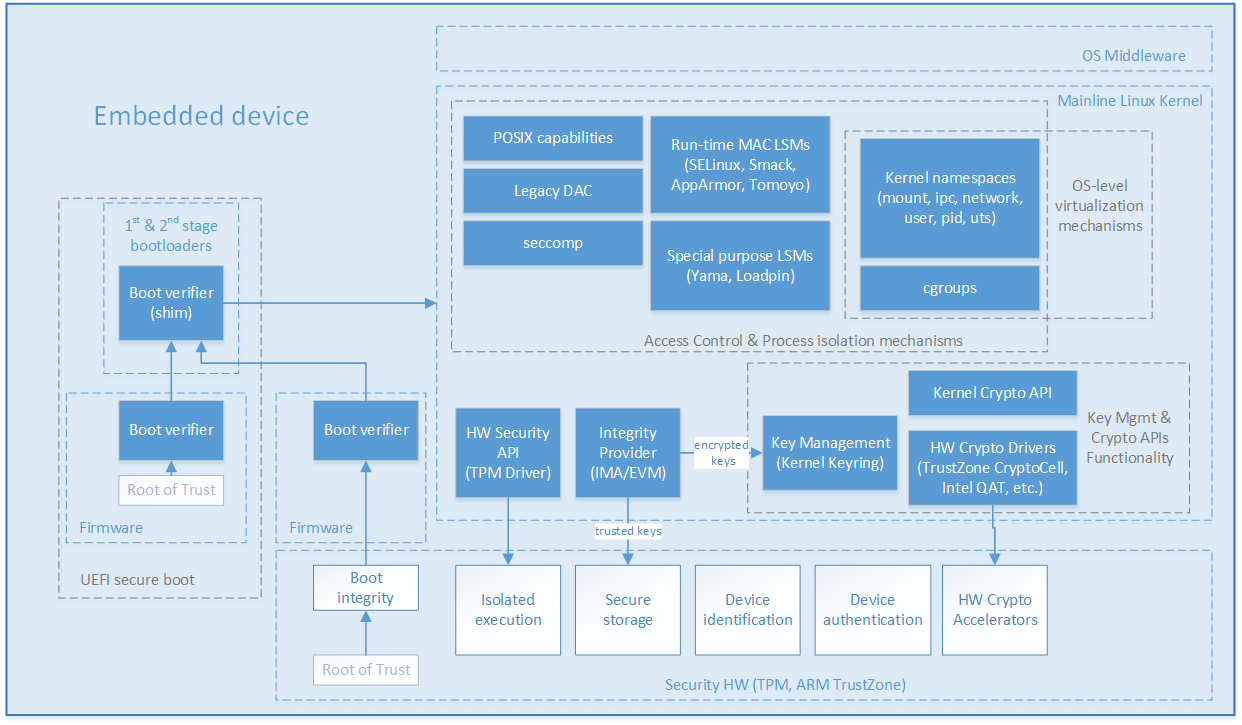
\includegraphics[width=1\textwidth]{figures/LinuxKernelPlatSecModel.png}
	\caption{Platform Security Model for an Embedded device based on mainline Linux}
	\label{fig:platsec}
\end{figure}

If present, the \textit{Security HW} layer can be implemented using many existing technologies, such as Trusted Platform Module (TPM)~\cite{tpm}, ARM TrustZone~\cite{trustzone}, etc. In order to communicate with this layer, one needs to provide a \textit{Security HW API}, which is usually done in the form of a custom Linux driver. For example, the mainline Linux kernel has a TPM driver~\cite{tpmdriver} that provides an API to perform various operations supported by TPM Security HW. Regardless of the particular implementation details, there is a set of common elements that any typical Security HW provides:

\begin{itemize}
	\item \textbf{Root of Trust}. \textbf{Secure boot} is used to guarantee that the device configuration (firmware and software) hasn't been altered from its original trusted state even when device is in the offline state. This is typically done by measuring each component of the device firmware and software stack and comparing the measures to the signed reference values. Should the comparison fail, the boot can be either aborted (true "secure boot") or continued, but with some measures taken to protect the secrets residing inside Security HW ("authenticated boot"). However, in order for this system to work, one needs to start the measuring chain from an immutable \textbf{Root of Trust} that is safely stored inside the Security HW layer\footnote{If present, the HW Root of Trust can be used for many other purposes in addition to the secure boot, such as derivation of keys, secure storage, etc.}. Alternatively, it is possible to implement the secure boot without the support of the security HW, like is done in the \textbf{UEFI Secure boot} mechanism~\cite{uefi}. In this case, the root of trust is embedded directly into the device firmware image.
	\item \textbf{Isolated execution} is another important element that is used to execute the security-critical code that should not be observable in any way by potentially malicious OS or applications. This element is also commonly referred to as \textbf{Trusted Execution Environment} (TEE).
	\item \textbf{Secure Storage} functionality can be used by different OS components in order to guarantee data integrity and confidentiality even in the presence of offline attacks. For example, if TPM module is present on a device, the Integrity Measurement Architecture (IMA) component~\cite{ima}, described below in more detail, uses TPM's secure storage functionality to guarantee security of its \textit{trusted keys}.
	\item \textbf{Device identification and authentication}. Embedded devices might need to have unique identifiers that can be used for different purposes, such as immutable MAC addresses, automotive identifiers, etc.  Additionally it should be possible for a device to reliably prove its identity to an external party, which is typically done in the form of a process called "\textit{remote attestation}". For example this might be needed in order to get access to some external services or receive platform updates.
	\item \textbf{HW Crypto Accelerators} can be used in order to significantly speed up the costly cryptographic computations and in Linux are accessible via dedicated \textit{HW Crypto drivers}, such as TrustZone CryptoCell~\cite{cryptocell} or Intel Quick Assist Technology~\cite{intelQAT} cryptographic drivers.
\end{itemize}

The mainline Linux kernel itself has a number of platform security mechanisms that aim at addressing different security requirements. The biggest group of such mechanisms provides ways for implementing \textit{process and application isolation} on a device by means of a run-time access control. These mechanisms differ greatly in the level and type of access control they provide, depending not only on the mechanism itself, but also on its associated policy or configuration:

\begin{itemize}
	\item \textbf{POSIX capabilities}~\cite{caps} is a set of permissions that can be granted to a process in order to perform a defined system function. For example, a \setype{CAP\_NET\_ADMIN} capability allows a process to perform various privileged network-related operations, like administration of network interfaces and routing tables, access to advanced socket configuration settings, etc. By default the Linux superuser ("root" user with user id 0) possesses all defined capabilities, while other users have none, but it is possible to create different configurations using the \textit{file capabilities} feature~\cite{filecaps}. 
	\item The \textbf{Legacy Discretionary Access Control (DAC) mechanism}, initially developed decades ago for separating different device users and their data, is still present and functioning as originally, but since most present-day devices are single-user, it is used instead for separating processes and groups of processes. For example, the Android mobile OS uses Linux DAC mechanisms for implementing its permission model. The main downside of DAC is the lack of a centralized access control policy that can be enforced device-wise, because each data owner can freely grant access to its data to other processes. 
	\item This gap is addressed by \textbf{Mandatory Access Control (MAC)} mechanisms that in the mainline Linux kernel implemented in a form of \textit{Linux Security Modules (LSM)}, such as SELinux~\cite{smalley2001implementing}, AppArmor~\cite{bauer2006paranoid}, Smack~\cite{bauer2006paranoid} and Tomoyo~\cite{tomoyo}. They allow defining a unified access control policy for the whole device that can be formally analyzed for allowed information flows, conflicts, etc. MAC LSMs are very powerful access control mechanism in Linux and it is actively used on the systems with strict security requirements for run-time process isolation, such as enterprise servers and mobile devices. 
	\item In addition to MAC LSMs the mainline Linux kernel has \textbf{special-purpose LSMs}, Yama~\cite{yama} and Loadpin~\cite{loadpin}, that do not provide a system-wide MAC mechanism, but instead serve a much narrower focus of limiting process abilities. For example, Yama LSM allows limiting the dangerous Linux process tracing feature, where a (potentially compromised) process can examine the memory and running state of any other process running under the same user identifier. 
	\item \textbf{Seccomp}~\cite{seccomp2016} is another special purpose mechanism that allows a process to restrict the ability to make system calls to a smaller set specified using a seccomp filter. This can be useful if a process performs little system calls after the initialization stage and, should it get compromised later on, the compromised process abilities are significantly limited.
\end{itemize} 

Recently two additional mechanisms, initially developed to support OS-level process virtualization, have started to be used for application isolation on Linux: \textbf{Kernel namespaces}~\cite{biederman2006} and \textbf{cgroups}~\cite{cgroupsv2}. These mechanisms, described in more detail in Section~\ref{sec:os-virt} of this thesis, allow a process to have its own limited virtualized view of the system to which it is confined and cannot escape from. However, there is a constant debate in the Linux security community about the security level that these mechanisms provide and the appropriate way of using them.   

The mainline Linux kernel also provides a \textbf{Key Management} (\textbf{Kernel Keyring}~\cite{keyrings}) and \textbf{Kernel Crypto API}~\cite{kernelcryptoapi} components. They can be used to generate and store keys and other credentials, and to perform various cryptographic operations, such as signing, encryption, hashing etc. The set of available algorithms consists of a set implemented within the kernel, as well as additional algorithms that might be provided by Security HW and exposed via \textit{HW Crypto Drivers} described above.

The last remaining mechanism, \textbf{Integrity Measurement Architecture} (IMA)~\cite{ima}, and its extension, \textbf{Extended Verification Module} (EVM)~\cite{ima}, can be used to extend the secure boot and guarantee the offline integrity of the userspace layer and filesystem. IMA/EVM does this by calculating a hash over each file before it is accessed and comparing this hash with a reference value stored in the file's signed extended attributes. IMA/EVM supports two types of keys: \textit{trusted} and \textit{encrypted}. The former depend on Security HW (such as TPM) being present on the system and stored within its secure storage facilities, while the latter ones can always be used and stored in the Kernel Keyring component. 

Out of all platform security mechanisms described above, the process and application isolation methods are ultimately the hardest ones to configure and use correctly. Not only does the mainline Linux kernel have multiple options that can be used simultaneously, but each of these options provides unlimited ways of how it can be configured. This is very challenging given that the end security of such mechanisms fully depends on their configuration or policy, which might be at best provided only in a reference policy form and only for certain limited use cases. For example, there is a SELinux reference policy for Fedora desktop that only covers the packages included in the Fedora distribution, but as soon as new packages are added or substituted (common in the case of embedded devices), the policy needs adjustments and additions. Therefore the first main focus of the thesis, described in Chapter~\ref{sec:ac-policies}, is the method for process isolation and access control, where we will take a look on the typical challenges of building secure MAC policies, as well as propose methods and tools that can help in the process. We will also focus on alternative mechanisms for achieving process and application isolation by using OS-level virtualization methods. 

In addition to the above described mechanisms, there is an area that has recently gained a lot of focus in the mainline Linux security community, namely the OS kernel protection against run-time exploits. The importance of this direction cannot be underestimated since a successful attack on the OS kernel itself renders all of its security mechanisms ineffective and useless. Therefore the second main focus of the thesis, described in Chapter~\ref{sec:kernel-hardening}, is the OS Kernel Hardening, where we will discuss the overall ways to enhance the run-time exploit protection of the mainline Linux kernel, as well as present concrete mechanisms for achieving this goal. 
 